\documentclass[11pt,a4paper]{report}

\usepackage{graphicx}
\usepackage{epstopdf}
\usepackage[section]{placeins} % 'one-shot' command to nicely place figures
\usepackage{datatool}
\usepackage{url}
\DeclareUrlCommand\UScore{\urlstyle{rm}}



\newcommand{\anuga}{\textsc{anuga}}


\newcommand{\inputresults}[1]{\graphicspath{{#1/}}
\section{Dam Break}

Standard dam break test problem. Should show rarefaction fan and shock. 

\subsection{Results}


We should see excellent agreement between the analytical and numerical solutions.

\begin{figure}[h]
\begin{center}
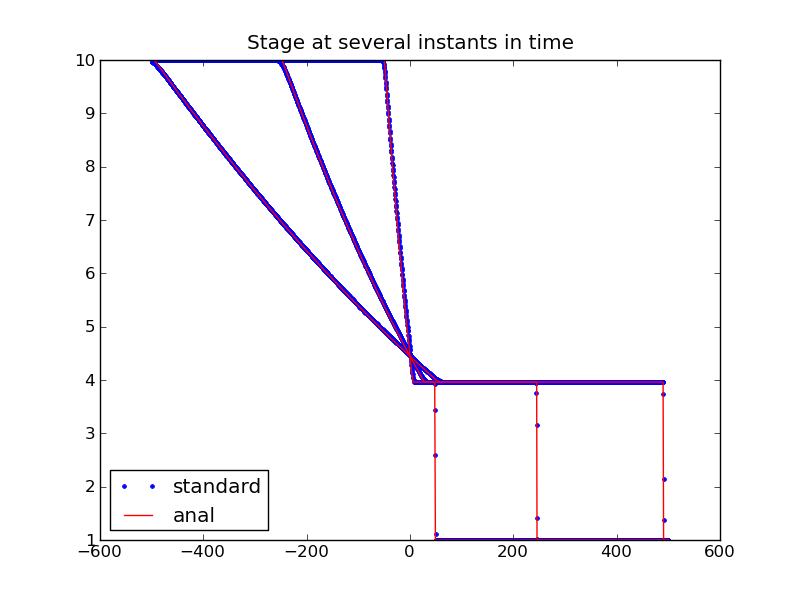
\includegraphics[width=0.9\textwidth]{stage_plot.png}
\end{center}
\caption{Stage results}
\end{figure}


\begin{figure}[h]
\begin{center}
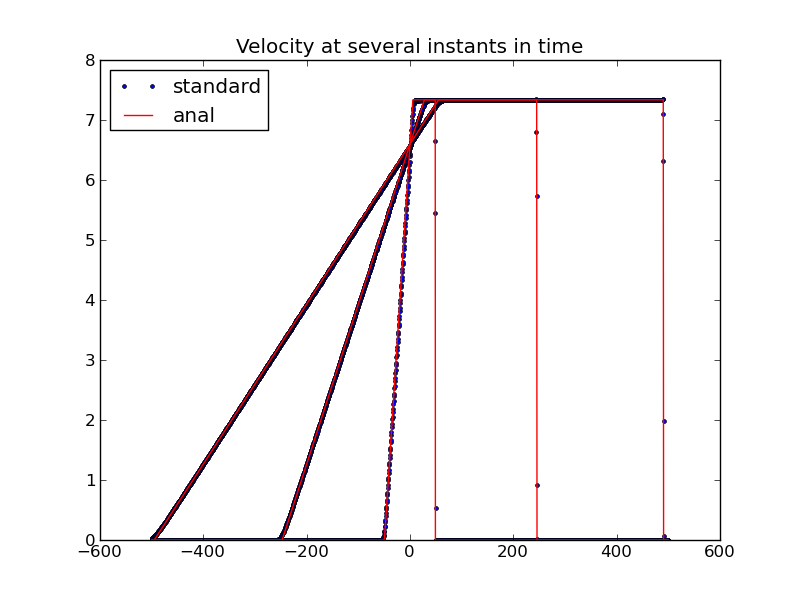
\includegraphics[width=0.9\textwidth]{xvel_plot.png}
\end{center}
\caption{Velocity results}
\end{figure}


\endinput
}
\newcommand{\cfl}{\UScore{1.0}}
\newcommand{\alg}{\UScore{tsunami}}
\newcommand{\majorR}{\UScore{1.3.0_beta}}
\newcommand{\minorR}{\UScore{8581}}
\newcommand{\timeR}{{Tue Sep 18 15:39:06 2012}}


%=========================================
\begin{document} 
%=========================================

\title{Automated Report on the Performance of \anuga ~on Various Test Problems}
\maketitle
\tableofcontents

%======================
\chapter{Introduction}
%======================

The results in this report were produced by \anuga{} version \majorR{} 
from svn repository revision \minorR{} at time \timeR.
The flow algorithm was \alg{} and cfl condition \cfl.

%======================
\chapter{Analytical Tests}
%======================

\inputresults{Tests/Analytical/Dam_Break}

\inputresults{Tests/Analytical/runup1}

\inputresults{Tests/Analytical/runup_sinusoid}

\inputresults{Tests/Analytical/trapezoidal_channel}

\inputresults{Tests/Analytical/parabolic_basin_1D}

\inputresults{Tests/Analytical/deep_wave}

\inputresults{Tests/Analytical/steep_slope}

%======================
\chapter{Experimental Tests}
%======================

\inputresults{Tests/Experimental/Isolated_Building}

%======================
\chapter{Real World Tests}
%======================

\inputresults{Tests/Real_World/Patong}

%======================
\appendix
%======================
%======================
\chapter{Adding New Tests}
%======================


To setup a new validation test, create a test directory under the
\textsc{Tests} directory. In that directory there should be the test code, a
\TeX{} file \texttt{results.tex} and a python script
\texttt{produce\_results.py}, which runs the simulation and produces the
outputs. In this \TeX{} file, \texttt{report.tex}, add a line
\begin{verbatim}
\inputresults{Tests/Directory/Name}
\end{verbatim}



\section{Specifiying different algorithm}
One  way to allow the system to run with different algorithms is to add the following
into your run routines.
\begin{verbatim}
#--------------------------------
# Setup Default values for basic
# algorithm parameters.
#--------------------------------
import argparse
parser = argparse.ArgumentParser(description='produce results')
parser.add_argument('-cfl', type=float, default=1.0,
                   help='cfl condition')
parser.add_argument('-alg', type=str, default = "1_5",
                   help='flow algorithm')
args = parser.parse_args()

cfl = args.cfl
alg = args.alg
\end{verbatim}

Then in the \texttt{produce\_results.py} you can 

\end{document}
